\documentclass[10pt]{beamer}
\usetheme{m}
\metroset{background=light}
\metroset{everytitleformat=regular}

\usepackage{fontspec}
\usepackage[math-style=TeX]{unicode-math}

%\usepackage[dvipdfmx]{multimedia}
\usepackage[dvipdfmx,final]{media9}

\usepackage{graphicx}
\graphicspath{{.}{assets/}}

\usepackage{xcolor}
\definecolor{pPurple}{HTML}{EA00FF}
\definecolor{pRed}{HTML}{FF0000}
\definecolor{pOrange}{HTML}{EB811B}
\definecolor{pGreen}{HTML}{1E6A1E}

\setbeamertemplate{caption}{\raggedright\insertcaption\par}

\title{Photometry of Bright B Stars using Contaminated \textit{Kepler}/K2 Pixels}
\author{Aleksa Sarai}
\date{\today}
\institute{SIfA --- University of Sydney}

\begin{document}
	\maketitle

	\begin{frame}{\textit{Kepler} and the K2 Mission}
		\begin{overlayarea}{\textwidth}{.3\textheight}
			\begin{itemize}
				\item Sent up in 2009, to scan a particular field.
				\item \dots until it malfunctioned in 2013 (\textit{oops!}).
				\item Repurposed to do \textbf{awesome} science on new fields.
				\item One of the greatest telescopes in history.
			\end{itemize}
		\end{overlayarea}

		\vfill

		\begin{figure}
			\centering
				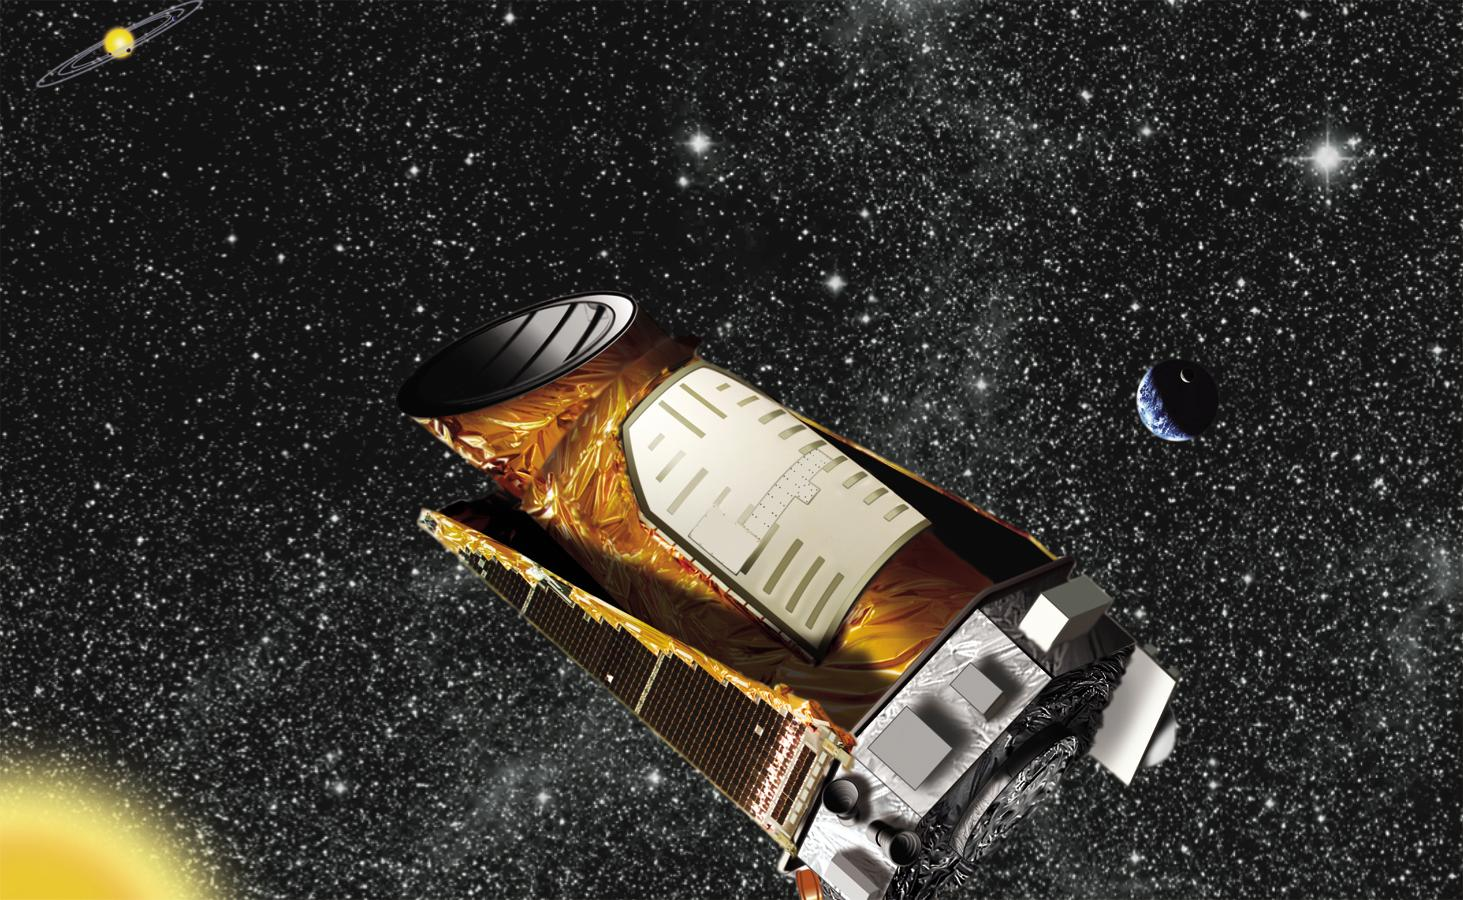
\includegraphics[height=.5\textheight,width=\textwidth,keepaspectratio]{kepler}
		\end{figure}
	\end{frame}

	\begin{frame}{Asteroseismology and Photometry}
		\begin{overlayarea}{\textwidth}{.5\textheight}
			\begin{figure}
				\centering
					\includemedia[
						activate=pageopen,
						width=.5\textheight,
						height=.5\textheight,
						addresource=assets/oscillations.mp4,
						flashvars={%
							source=assets/oscillations.mp4%same path as in addresource!
							&autoPlay=true%optional configuration
							&loop=true%variables
						}
					]{}{VPlayer.swf}
			\end{figure}
		\end{overlayarea}

		\vfill

		\begin{itemize}
			\item Stars aren't static --- they show variability.
			\item \textbf{Asteroseismology}: study of variability to probe inside stars.
			\item \textbf{Photometry}: counting photons to do \textit{asteroseismology}.
			\item Traditionally believed photometry requires all flux from target.
		\end{itemize}
	\end{frame}

	\begin{frame}{Why Bright Stars?}
		\begin{itemize}
			\item We like bright stars!
			\item Nearby and well studied.
			\begin{enumerate}
				\item Improve existing models.
				\item No good data for these targets (for quite a while yet).
				\item Follow-up research from the ground.
			\end{enumerate}
			\item But, bright star photometry is hard.
		\end{itemize}
	\end{frame}

	\begin{frame}{Bandwidth Issues}
		\begin{overlayarea}{\textwidth}{.5\textheight}
			\begin{figure}
				\centering
					\includegraphics[height=.45\textheight,width=\textwidth,keepaspectratio]{k2_ffi}
			\end{figure}
		\end{overlayarea}

		\vfill

		\begin{itemize}
			\item Limited bandwidth as \textit{Kepler} is very far away and covers a large field of view.
			\item Provide ``postage stamps'' ($\approx30000$) --- small cutouts around chosen targets taken every 30 minutes.
			\item Bright stars require bigger cutouts and thus more bandwidth.
			\item {\Large $\therefore$} No postage stamps of bright stars.
		\end{itemize}
	\end{frame}

	\begin{frame}{What if \dots}
		\begin{itemize}
			\item<2-> \dots postage stamps we \textbf{do} have could be used to do photometry on bright stars \textbf{without} postage stamps?
			\item<3-> \dots there are targets close enough to bright stars such that the flux \textit{contaminates} the postage stamp?
			\item<4-> \dots we could do photometry on \textbf{ALL THE THINGS}?
		\end{itemize}
	\end{frame}

	\begin{frame}{Contamination}
		\begin{overlayarea}{\textwidth}{.5\textheight}
			\begin{figure}
				\centering
					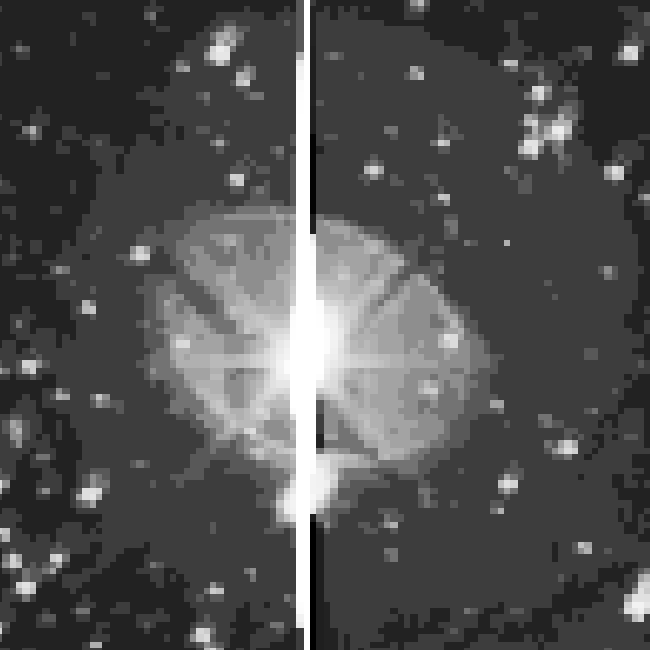
\includegraphics[height=.5\textheight,width=.5\textwidth,keepaspectratio]{k2_pointspread_large}
			\end{figure}
		\end{overlayarea}

		\vfill

		\begin{itemize}
			\item CCD sensors work by counting electrons ejected by photons in each pixel.
			\item Photons are scattered, internally reflected and defracted, causing a halo.
			\item Subset of halo pixels have a proportional photon count.
			\item {\Large $\therefore$} Photometry can be done using subset of halo pixels.
		\end{itemize}
	\end{frame}

	\begin{frame}{Normal}
		\begin{figure}
			\centering
				\only<1>{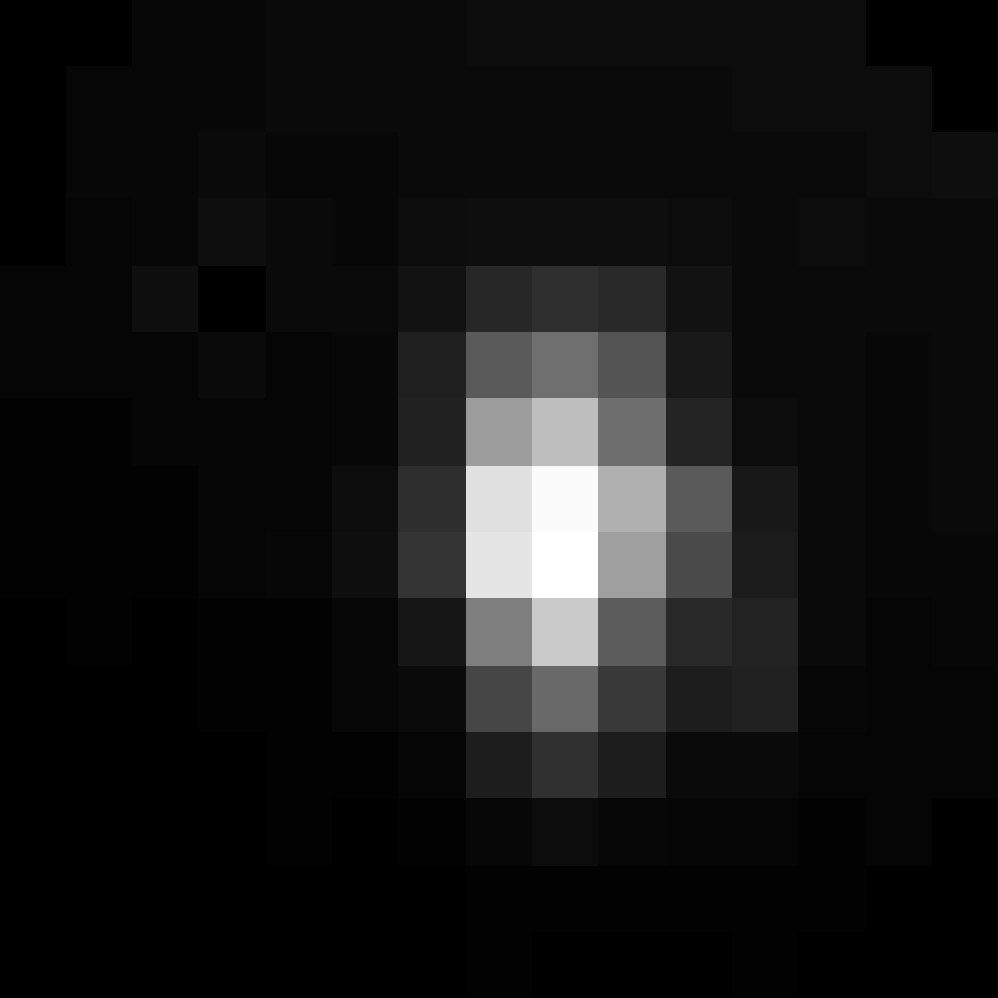
\includegraphics[height=.8\textheight,width=.8\textwidth,keepaspectratio]{k2_normal}}
				\only<2>{
\includegraphics[height=.8\textheight,width=.8\textwidth,keepaspectratio]{k2_normal_overlay}}
			\caption{\textit{Kepler}/K2: Normal (\textit{\textbf{aka} boring}) postage stamp.}
		\end{figure}
	\end{frame}

	\begin{frame}{Contaminated}
		\begin{figure}
			\centering
				\only<1>{
\includegraphics[height=.8\textheight,width=.8\textwidth,keepaspectratio]{k2_contaminated}}
				\only<2>{
\includegraphics[height=.8\textheight,width=.8\textwidth,keepaspectratio]{k2_contaminated_overlay}}
			\caption{\textit{Kepler}/K2: Contaminated postage stamp.}
		\end{figure}
	\end{frame}

	\begin{frame}{Background}
		\begin{columns}[T,onlytextwidth]
			\begin{column}{.5\textwidth}
				\begin{figure}
					\centering
						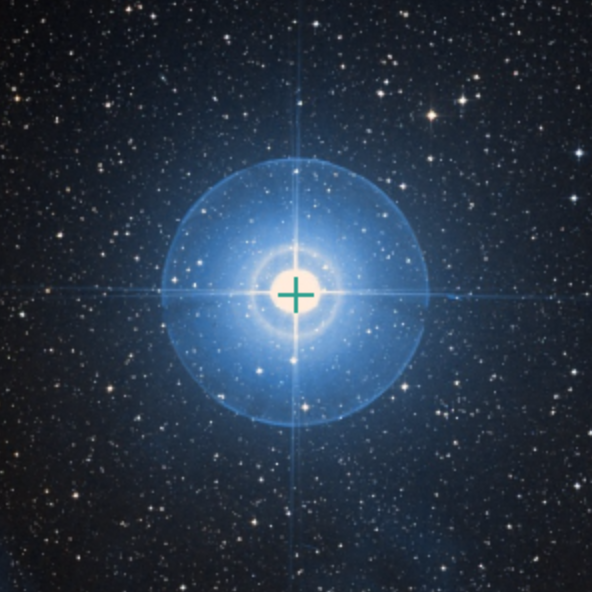
\includegraphics[width=\textwidth,keepaspectratio]{pi_sco_aladin}
					%\caption{\textit{AladinLite}: $\pi$ Sco.}
					\caption{\textit{Ground-based}: $\pi$ Sco.}
				\end{figure}
			\end{column}

			\begin{column}{.5\textwidth}
				\begin{minipage}[c][.6\textheight][c]{\linewidth}
					\begin{itemize}
						\item Scorpio constellation.
						\item $2.7$ magnitude (\textbf{very} bright --- can even be seen from Sydney!).
						\item Ellipsoidal binary, $T = 1.57 {\rm d}$.% \citep{schobbrook2005}.
						\item In the \textit{Kepler}/K2 field in \texttt{C02}.
					\end{itemize}
				\end{minipage}
			\end{column}
		\end{columns}
	\end{frame}

	\begin{frame}{Full Frame Image (K2)}
		\begin{figure}
			\centering
				\only<1>{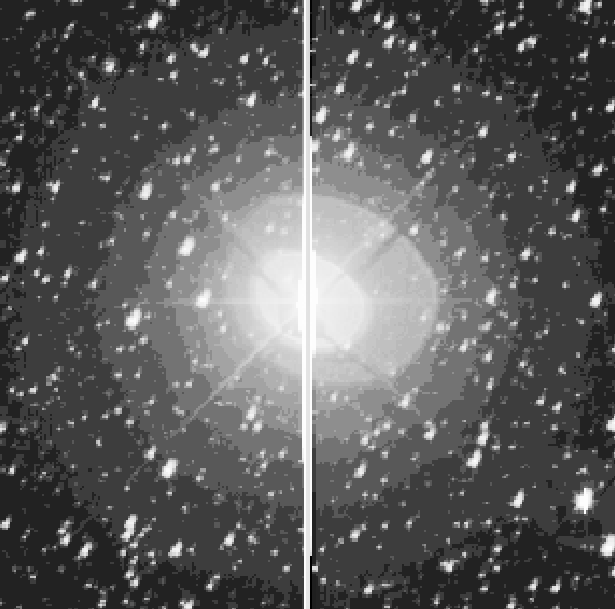
\includegraphics[height=.8\textheight,width=.8\textwidth,keepaspectratio]{pi_sco_k2raw}}
				\only<2>{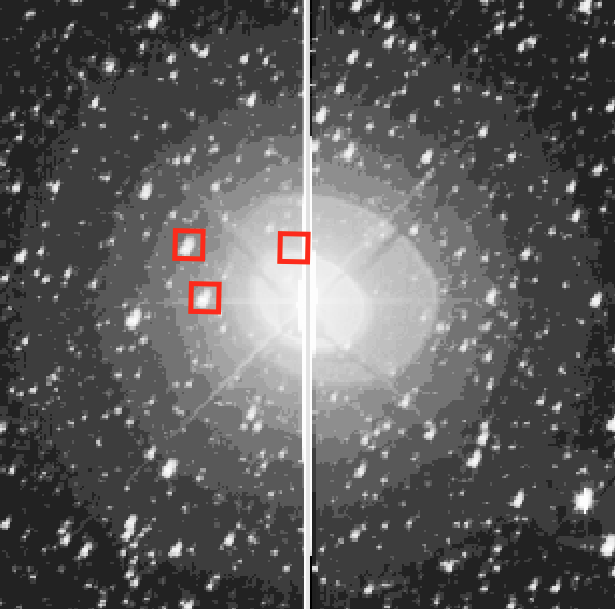
\includegraphics[height=.8\textheight,width=.8\textwidth,keepaspectratio]{pi_sco_k2overlay}}
			\caption{\textit{Kepler}/K2: $\pi$ Sco.}
		\end{figure}
	\end{frame}

	\begin{frame}{\tt EPIC 203442993}
		\begin{columns}[T,onlytextwidth]
			\begin{column}{0.5\textwidth}
				\begin{figure}
					\centering
						\begin{minipage}[c][\textwidth][c]{\textwidth}
							\only<1>{\includemedia[
								activate=pageopen,
								width=\textwidth,
								height=\textwidth,
								addresource=assets/pi_203442993_k2animated.mp4,
								flashvars={%
									source=assets/pi_203442993_k2animated.mp4%same path as in addresource!
									&autoPlay=true%optional configuration
									&loop=true%variables
								}
							]{}{VPlayer.swf}}
							\only<2>{
\includegraphics[width=\textwidth,keepaspectratio]{pi_203442993_k2overlay}}
						\end{minipage}
					\caption{\textit{Kepler}/K2: \texttt{EPIC 203442993}.}
				\end{figure}
			\end{column}

			\begin{column}{0.5\textwidth}
				\begin{minipage}[c][.6\textheight][c]{\linewidth}
					\begin{enumerate}
						\item Follow motion.
						\item Mask contaminated pixels.
						\item Sum flux in mask for each frame.
					\end{enumerate}
				\end{minipage}
			\end{column}
		\end{columns}
	\end{frame}

	\begin{frame}{Our Analysis}
		\begin{figure}
			\centering
				\only<1>{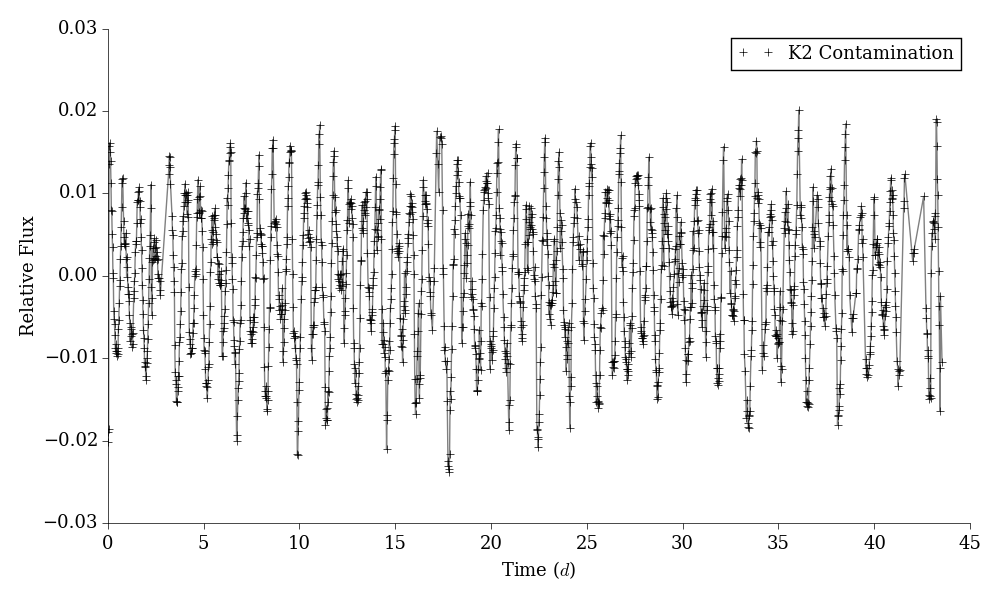
\includegraphics[width=\textwidth,keepaspectratio]{pi_sco_lc_k2_raw}}
				\only<2>{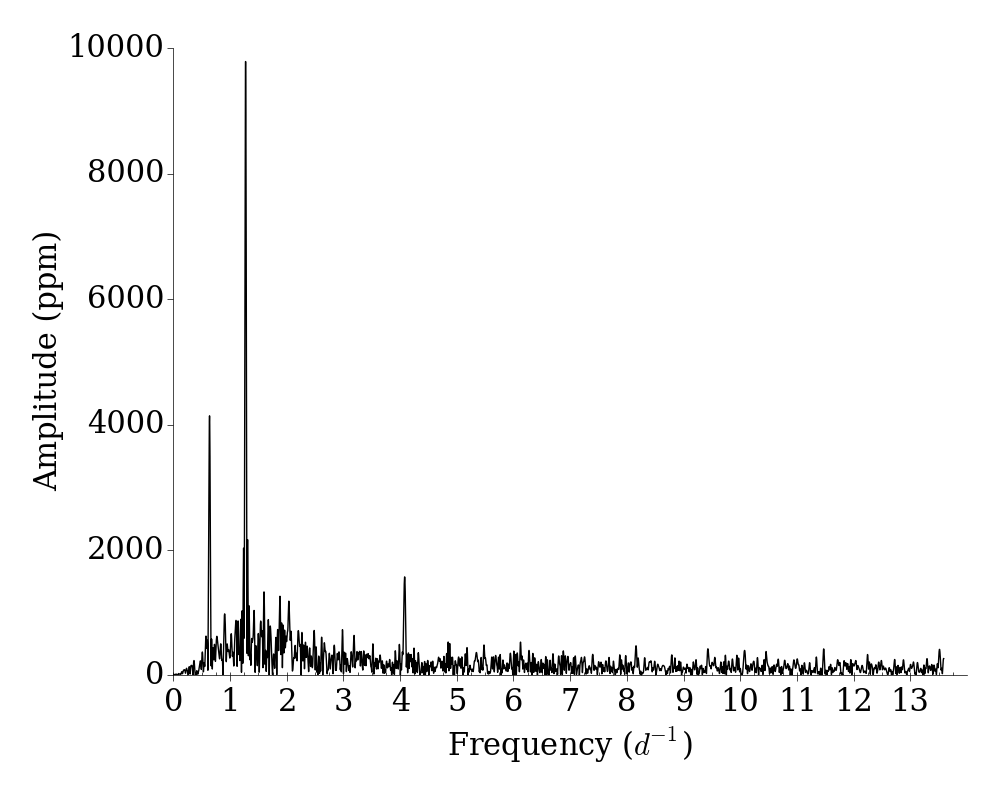
\includegraphics[width=\textwidth,keepaspectratio]{pi_sco_lc_k2_fft}}
				\only<3>{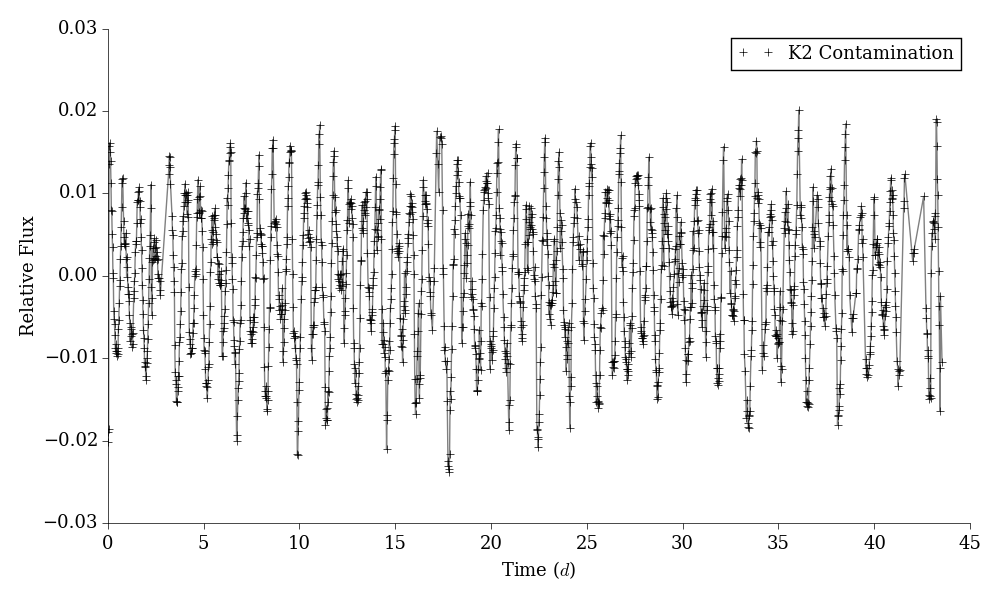
\includegraphics[width=\textwidth,keepaspectratio]{pi_sco_lc_k2_raw}}
				\only<4>{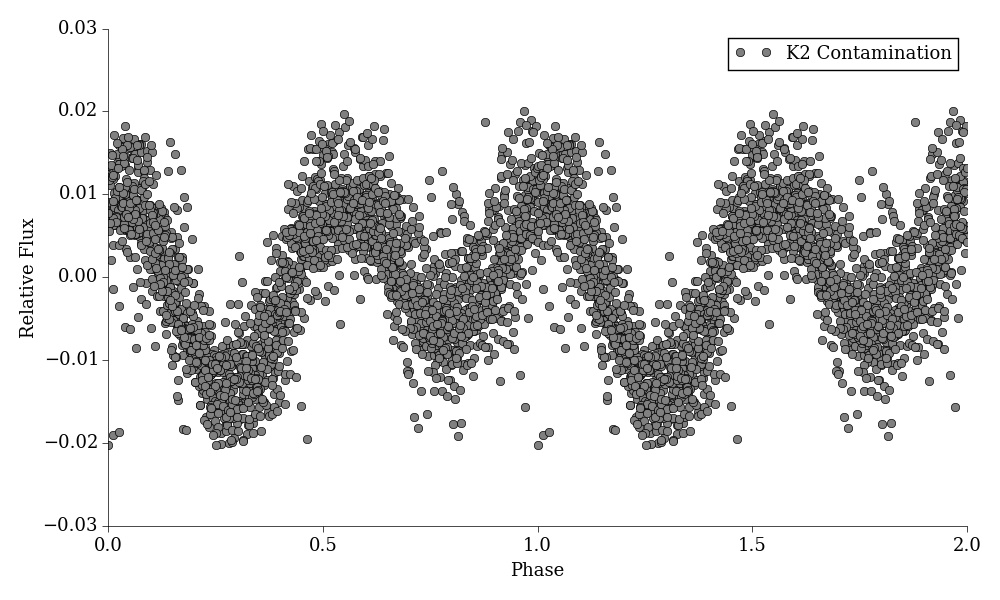
\includegraphics[width=\textwidth,keepaspectratio]{pi_sco_lc_k2}}
		\end{figure}
	\end{frame}

	\begin{frame}{Previous Surveys}
		\begin{overlayarea}{\textwidth}{.75\textheight}
			\begin{figure}
				\centering
					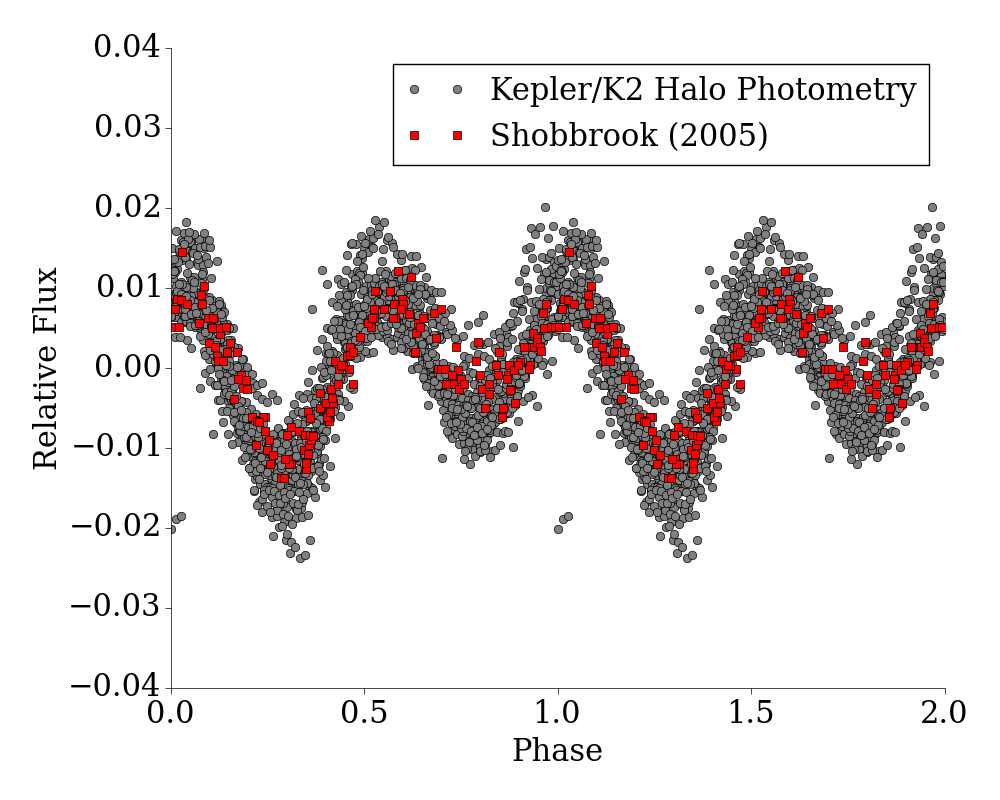
\includegraphics[width=\textwidth,keepaspectratio]{pi_sco_lc_both}
			\end{figure}
		\end{overlayarea}

		\begin{itemize}
			\item Shobbrook (2005) photometric analysis of $\pi$ Sco, from ground with \textbf{10 year} baseline.
		\end{itemize}
	\end{frame}

	\begin{frame}{Future Research}
		\begin{itemize}
			\item Wrapping up:
			\begin{enumerate}
				\item Reproduced ground-based data.
				\item Shown contamination photometry is viable.
				\item Did in 45 days what took Shobbrook 10 years (with more data).
			\end{enumerate}
			\item More postage stamps, from more campaigns.
			\item Do new science with data otherwise neglected.
			\item Investigate improvements to technique.
		\end{itemize}
	\end{frame}

	\begin{frame}{Acknowledgements}
		\begin{itemize}
			\item Thanks to my supervisors:
			\begin{itemize}
				\item Tim Bedding
				\item Daniel Huber
				\item Simon Murphy
			\end{itemize}
			\item \dots and to some other researchers, whose help was also invaluable:
			\begin{itemize}
				\item Benjamin Pope
				\item Tim White
			\end{itemize}
			\item \dots and the Talented Student Program organiser Helen Johnston.
		\end{itemize}
	\end{frame}

	\section{Questions?}
\end{document}
